\hypertarget{development-process}{%
\chapter{Development Process}\label{development-process}}

\hypertarget{kanban}{%
\section{Kanban}\label{kanban}}

To keep track of tasks we used a Kanban board on Github.


\begin{figure}[H]
\centering
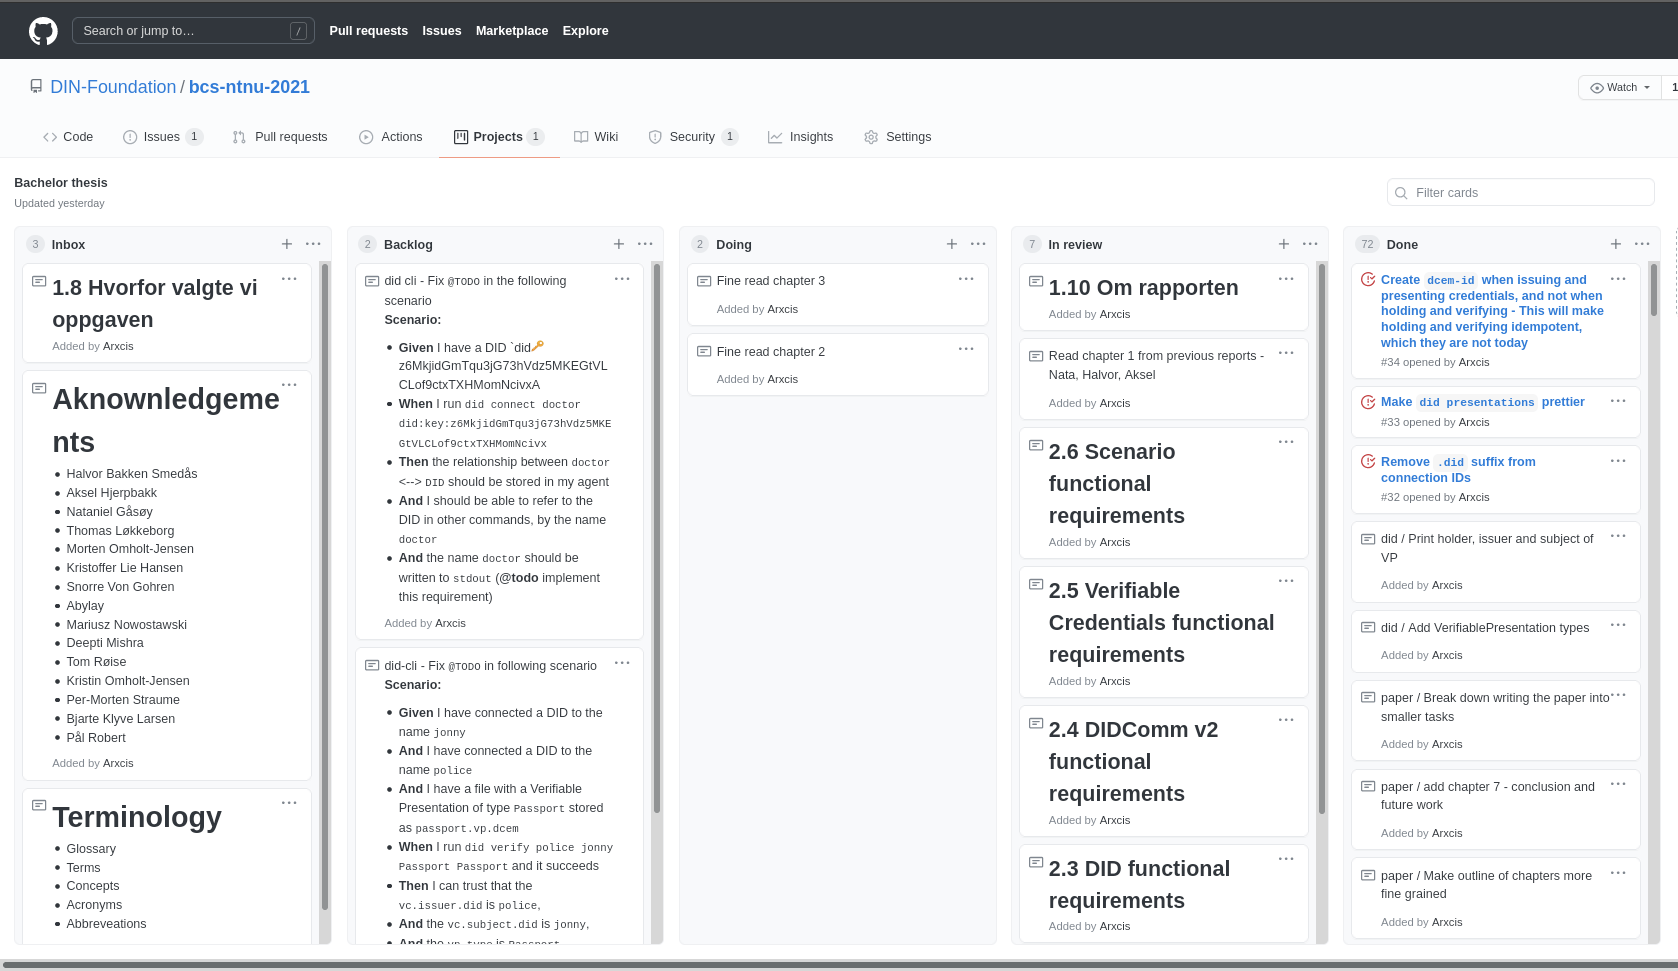
\includegraphics[width=\textwidth]{Development Process a132dd5987b94adf8fc5989add9afc3f/Untitled.png}
\caption{Kanban on Github}
\end{figure}




% ############################################################################
% ------------------------------- PAGE BREAK -----------------------------------
% ############################################################################
\pagebreak




\hypertarget{the-5-columns-of-the-kanban-board}{%
\subsection{The 5 columns of the Kanban
board}\label{the-5-columns-of-the-kanban-board}}

\begin{enumerate}
\def\labelenumi{\arabic{enumi}.}
\tightlist
\item
  \textbf{Inbox:} List of tasks which have been thought of, but is
  lacking details like what needs to be done and when the implementation
  is supposed to happen. Tasks in backlog are created whenever someone
  feels like it. There are no requirements to put something in the
  backlog. The treshold should be as low as possible. Eqaully, the
  treshold for deleting a backlog-task should be equally low.
\item
  \textbf{Backlog:} List of tasks that are planned to be implemented in
  the near future, and have enough details ironed out to make it
  possible to start the implementation. Tasks are moved from
    \textit{Inbox} to \textit{Backlog}:

  \begin{enumerate}
  \def\labelenumii{\arabic{enumii}.}
  \tightlist
  \item
    After being discussed in the weekly domain-experts meeting.
  \item
    item or after an ad-hoc meeting dedicated to discussing a specific
    task.
  \item
    item or after the developer has researched/learned something which
    makes a task ``obviously implementable''. If a developer does this,
    it should be clearly communicated in the next weekly domain-experts
    meeting.
  \end{enumerate}
\item
  \textbf{In Progress}: List of tasks that are in progress. A developer
  have written words, code or done something else. These tasks should
  ideally be linked to an open Pull Request on Github with a WIP label
  on it.
\item
  \textbf{In Review:} List of tasks where the developer has implemented
  the task, and is waiting to get a stamp of approval from a second pair
  of eyes. Approval could be given by the client, supervisor or any of
  the domain experts. The developer will request review from the
  specific person which is considered best suited to review the pull
  request. This specific person will be notified about this on Discord,
  and via email if necessary.
\item
  \textbf{Done:} List of task where the pull request linked to the task
  has been approved and merged into the main branch of the git source
  tree.
\end{enumerate}


\hypertarget{github-source-code}{%
\section{Github source code}\label{github-source-code}}

All source code is hosted at
\url{https://github.com/DIN-foundation/bcs-ntnu-2021/}.

\hypertarget{source-code-of-did-cli}{%
\subsection{Source code of DID-CLI}\label{source-code-of-did-cli}}

All DID-CLI source code was kept in a public open-source Github-repo,
during the entire development. This made it easier to collaborate on the
source code, because all participants had public access to all the work
that was being done, from day one, including members Decentralized Identity Foundation (DIF).

\begin{figure}
\centering
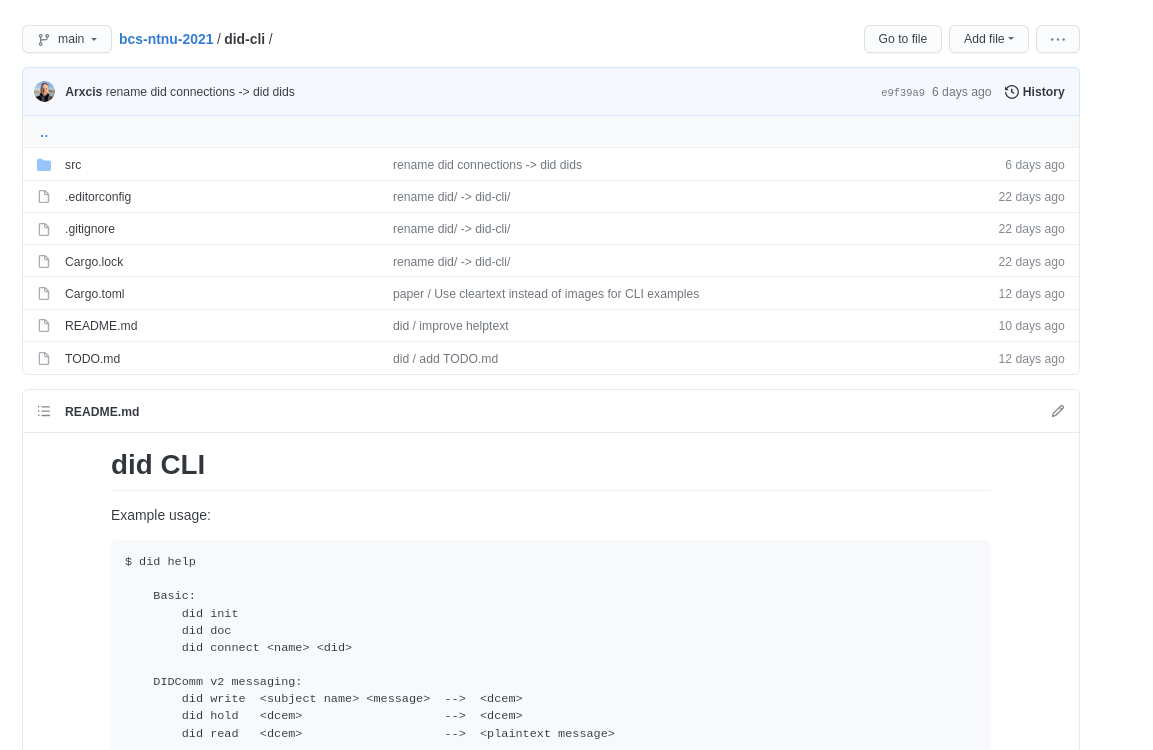
\includegraphics[width=\textwidth]{Development Process a132dd5987b94adf8fc5989add9afc3f/Untitled 1.png}
\caption{Untitled}
\end{figure}



% ############################################################################
% ------------------------------- PAGE BREAK -----------------------------------
% ############################################################################
\pagebreak



\hypertarget{source-code-of-playground-example}{%
\subsection{Source code of Playground
examples}\label{source-code-of-playground-example}}

Before implementing the DID-CLI, a lot of experimentation had to be
done. This was done to learn, and iterate on smaller projects, before
beginning on the big one. Most of the projects in \textit{/playground}
are useless, but they served an important role as learning exercises.


\hypertarget{source-code-of-report}{%
\subsection{Source code of Report}\label{source-code-of-report}}

Even the report was initially developed on Github, in the same repo as
DID-CLI and playground.


\hypertarget{weekly-meetings}{%
\section{Weekly meetings}\label{weekly-meetings}}

\hypertarget{weekly-meeting-notes-on-github}{%
\subsection{Weekly meeting notes on
Github}\label{weekly-meeting-notes-on-github}}

Each meeting has a meeting note document attached to it, noting down the
attendees and a log of what was discussed during the meeting and can be
found here
\url{https://github.com/DIN-Foundation/bcs-ntnu-2021/tree/main/meetings}.




% ############################################################################
% ------------------------------- PAGE BREAK -----------------------------------
% ############################################################################
\pagebreak



\hypertarget{domain-experts-weekly---tuesdays-1230}{%
\subsection{Domain Experts Weekly - Tuesdays @
12:30}\label{domain-experts-weekly---tuesdays-1230}}

\begin{itemize}
\tightlist
\item
  \textbf{Agenda:} Discussed questions related to the problem-domain SSI
  and software engineering. Demonstrated and validated product
  iterations.
\item
  \textbf{Attendees}: Jonas, Snorre, Mariusz, Abylay.
\item
  \textbf{Where:} Google Meet
\end{itemize}

\hypertarget{academic-supervisor-weekly---wednesdays-1400}{%
\subsection{Academic Supervisor Weekly - Wednesdays @
14:00}\label{academic-supervisor-weekly---wednesdays-1400}}

\begin{itemize}
\tightlist
\item
  \textbf{Agenda:} Discussed everything related to academic writing and
  how to organize the project's workflow.
\item
  \textbf{Attendees:} Jonas, Deepti
\item
  \textbf{Where}: Microsoft Teams
\end{itemize}


\hypertarget{a-virtual-bachelor}{%
\subsection{A virtual bachelor}\label{a-virtual-bachelor}}

Due to the pandemic, all meetings were virtual. The team never got a
chance to meet in real life during the project period. Even the final
presentation of the bachelor thesis was given over MS teams. There is no doubt that this had an effect on how quickly the team was able to move project forward.


\hypertarget{community-servers}{%
\section{Community servers}\label{community-servers}}

\subsection{DIN Discord server}

During the development process many topics were discussed inside the
DINs Discord server. This is were most of the written technical
conversations between the team members took place.

\subsection{DIF Slack server}

After a long application process which started here
\url{https://identity.foundation/join/} , I was finally accepted as a
member of the DIF foundation and allowed access to their sacred Slack
server. Here you can find many of the authors and developers of the
different SSI standards, which was an invaluable resource during the
project.



% ############################################################################
% ------------------------------- PAGE BREAK -----------------------------------
% ############################################################################
\pagebreak



\hypertarget{toggl-time-tracking}{%
\section{Toggl Time Tracking}\label{toggl-time-tracking}}

Tracking the hours was done in Toggl from day 1 (week 5), and throughout
the project (end week 20). The hours were tagged with the following 6
categories:

\begin{itemize}
\tightlist
\item
  \textbf{Meeting:} Toggled when participating in a live meeting, or
  when writing meeting notes.
\item
  \textbf{Organizing:} Toggled when organizing meetings and creating and
  updating Kanban tasks.
\item
  \textbf{Writing}: Toggled when writing the bachelor report.
\item
  \textbf{Coding}: Toggled when coding in the playground mini-projects,
  or the DID-CLI main project.
\item
  \textbf{Researching}: Toggled when reading specifications, papers,
  blog-posts, discussing with experts on the DIF and DIN slack/Discord
  channels, watching videos, reading previous bachelor reports, reading
  books, and more\ldots{}
\item
  \textbf{Lecture}: Toggled when participating in weekly lectures in the
  profprog-course, or one of the ``lightning lectures'' related to the
  bachelor-course.
\end{itemize}


\begin{figure}
\centering
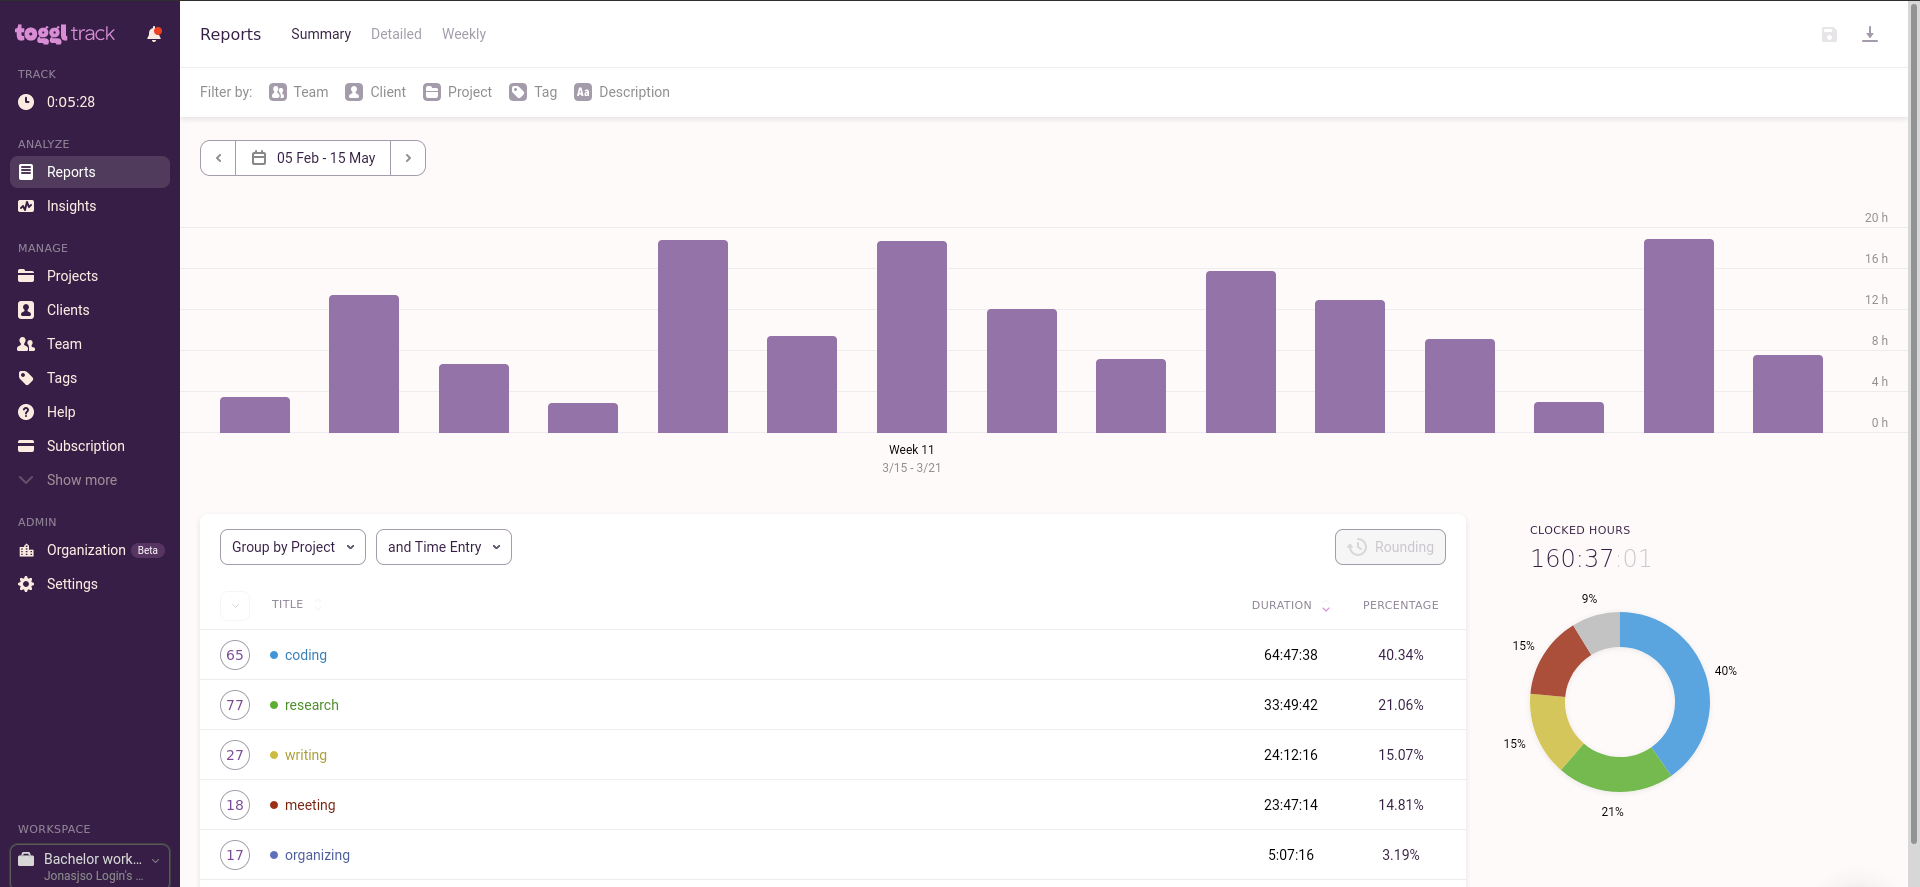
\includegraphics[width=\textwidth]{Development Process a132dd5987b94adf8fc5989add9afc3f/Untitled 6.png}
\caption{Toggl time tracking report from 05 Feb to 15 may}
\end{figure}
